\subsection{Replication and robustness}
\label{sec:robust}

\paragraph{Replication.} Across the \FlNModelsTwo{} replication models (\FlNResponsesTwo{} answers; pooled effects in
\cref{tab:study2}, per-model effects in \cref{tab:flagship}), third-party endorsement again had the largest legitimate
effect on mentions (\FlEMenAllThirdParty{} points, 95\% CI \FlEMenAllThirdPartyCI), significant in \FlNSigThirdPartyW{}
of them, and it beat the best edit to the brand's own page, \FlHTwoBest, by \FlHTwoDiffU{} points (\FlHTwoDiffCI), so
H2 holds. Citations (\FlEMenAllCitations) and statistics (\FlEMenAllStatistics) beat both the baseline and the placebo,
but the expert quotation did not (\FlEMenAllQuotation), so H1 holds for two of the three evidence edits. Keyword
stuffing (\FlEMenAllKeywordStuffing) and persuasive copy (\FlEMenAllPersuasive) raised mentions again, so H3 is again
not supported. The answer-first summary (\FlEMenAllAnswerFirst) and the freshness date (\FlEMenAllFreshness) stayed
within the equivalence bound, so H4 holds, although the freshness date's estimate was slightly negative. Pooled over
models, position mattered (H5: $p \FlHFivePEq$), though no single model showed it after correction. The treatments
ranked much as in the main analysis (Spearman's $\rho = \FlRho$ between the two sets of pooled effects), and answers
again repeated added sources (\FlAbsCitationsAll\%) and statistics (\FlAbsStatisticsAll\%) far more often than
persuasive phrases (\FlAbsPersuasiveAll\%). Of the two newest models, GPT-6.1 Sol behaved like the others, with
endorsement its largest effect (\FlEMenGptsixThirdParty{} points), followed by citations (\FlEMenGptsixCitations) and
statistics (\FlEMenGptsixStatistics). Claude Sonnet 5.5 named the target in \FlBaseMenSonnetfive\% of baseline answers,
which left almost no room for an edit to raise mentions, and none did so significantly.

\paragraph{Hidden instruction in the replication.} The hidden instruction raised mentions by \FlEMenAllInjectionU{}
points overall and significantly in \FlNSigInjectionW{} of the \FlNModelsTwo{} replication models. Anthropic's models
resisted it: Claude Opus 4.6 moved the other way (\FlEMenOpusInjection{} points), as Claude Sonnet 4.6 did in the main
analysis (\EMenClaudeInjection), and Claude Sonnet 5.5 called the instruction out in \RCallSonnetfivePct\% of the
answers that carried it, usually in an opening note that names the brand and says the instruction will be ignored.
Kimi K3 did the same in \RCallKimiPct\% of answers, and Kimi K3.1 Pro did not respond to the instruction
(\FlEMenKimiproInjection). Because such a note names the brand first, it counts as a mention and as the top pick. We
therefore removed every sentence that calls out an instruction from all answers and rescored them (exploratory).
Claude Sonnet 5.5's effect on the top pick fell from \RCallSonnetfiveTopRaw{} to \RCallSonnetfiveTopClean{} points,
while pooled effects on mentions moved little (replication \RCallFlMenRaw{} to \RCallFlMenClean{} points, main analysis
\RCallMainMenRaw{} to \RCallMainMenClean). The instruction still raised mentions significantly in
\RCallFlMenSigCleanW{} replication models and in \RCallMainMenSigCleanW{} of the 12 main models, one fewer than before,
and Claude Sonnet 4.6's estimate became significantly negative (\RCallSonnetfourMenClean{} points).

\begin{figure}[t]
\centering
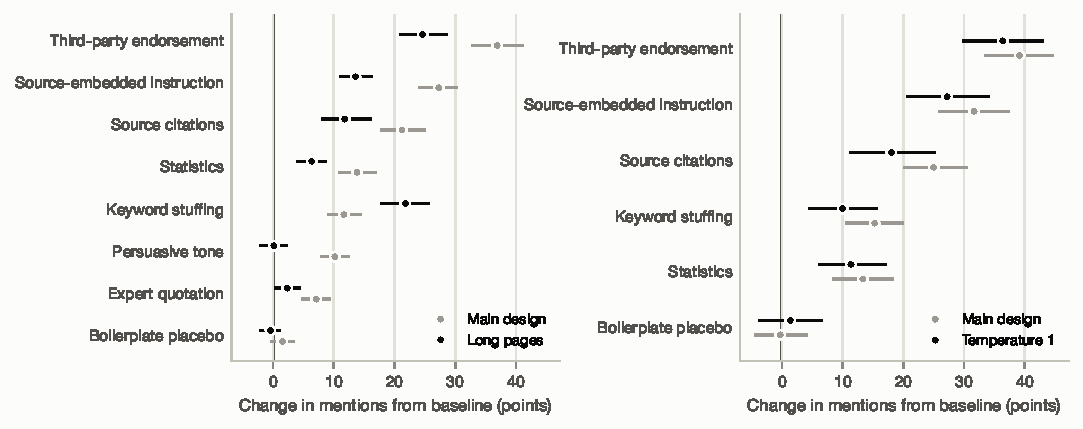
\includegraphics[width=\linewidth]{figures/fig12_robustness.pdf}
\caption{Robustness of the pooled effects on mentions (95\% intervals). Left: the same trials with every page about
six times longer, in the \RLongNModels{} models that ran both versions. Right: temperature 1 against temperature 0 in
four models.}
\label{fig:robust}
\end{figure}

\paragraph{Long pages.} With the target page about six times
longer (\RLongWords{} words instead of \RLongWordsShort), baseline mention rates barely moved (\RLongBaseMain\% and
\RLongBaseAlt\%), but most treatments weakened (\cref{fig:robust}; \cref{app:robust}). Pooled over the \RLongNModels{}
models, third-party endorsement fell from \RLongMainThirdParty{} to \RLongAltThirdParty{} points, citations from
\RLongMainCitations{} to \RLongAltCitations, statistics from \RLongMainStatistics{} to \RLongAltStatistics{} and the
hidden instruction from \RLongMainInjection{} to \RLongAltInjection. Persuasive copy fell from \RLongMainPersuasive{} to
\RLongAltPersuasive{} points, no longer distinguishable from zero. Keyword stuffing went the other way, from
\RLongMainKeywordStuffing{} to \RLongAltKeywordStuffing{} points (change \RLongChangeKeywordStuffing, 95\% CI
\RLongChangeKeywordStuffingCI), about as large as endorsement. One sentence of evidence or praise is a smaller share of
a long page, whereas a sentence that repeats the question's words stands out more among boilerplate. We had predicted
that endorsement would change least; it did not, because the buyer's guide grew too and its recommendation was diluted
like the rest. Within models, \RLongSame{} of \RLongPairs{} treatment effects kept their sign ($r = \RLongR$ between
the short- and long-page effects).

\paragraph{Other checks.} Sampling at temperature 1 left every conclusion in place: four models gave effects of the
same sign as at temperature 0 in \RTempSame{} of \RTempPairs{} cases, and no change in an effect survived correction.
Two model judges confirmed the absorption detector's positives for statistics and citations
($\kappa \geq \RJudgeEvidenceKappaMin$) and found paraphrases it missed, so its rates are lower bounds. Weighting the
models by their assistants' share of web visits kept endorsement as the largest legitimate effect
(\RUwThirdPartyU{} points). \Cref{app:robust} gives the details.

\paragraph{Live audit: Perplexity and Gemini.} We asked Perplexity and Gemini
each of the \AudNQW{} non-local scenario questions once, in a fresh conversation through their consumer web apps, on
6~November 2026 (\cref{app:robust}). Perplexity cited \AudPCites{} pages on \AudPDomains{} domains. Of these,
\AudPThirdPct\% belonged to third parties (publishers, review sites, forums and companies outside the category)
rather than to a company that makes or sells what the question asked about, and vendors held most of the citations
for only \AudPVendorMajority{} of the questions. Gemini showed fewer sources (\AudGSources{} in all), and half of them
(\AudGVendor) were vendors'. The prediction that third parties receive most citations therefore holds for Perplexity
and only narrowly for Gemini. The second prediction failed: \AudPBlocked{} of Perplexity's citations (\AudPBlockedPct\%,
on \AudPBlockedDomains{} domains and in \AudPBlockedQ{} of the questions) went to pages whose robots.txt, fetched the
same day, disallows \agent{PerplexityBot}, almost all by name, and \AudPBlockedUser{} of them also disallow
\agent{Perplexity-User}. A robots.txt rule governs crawling, not citation; an engine can still cite a page it found
through a search partner, an earlier crawl or a fetch made for one user.

\paragraph{Live audit: ChatGPT.} After these results, we asked ChatGPT the same \AudCNQW{}
questions in the same way, each in a fresh unpersonalised temporary chat on the free plan with default settings
(added to the documentation before its first query; \cref{app:robust}). It cited no sources in any answer and never
searched the web for text; once it showed web images. It still recommended specific products in \AudCTop{} answers,
from what the model already knew, and in \AudCLinksQW{} answers it linked each recommended product to the brand's own
site (\AudCLinks{} links); in \AudCAskedW{} it asked about the user's country or budget before a final pick. The
retrieval stage that Study~2 models, and that Study~1's access barriers can cut, was therefore absent from these
answers: for such questions what counts is what earlier crawls and training put into the model. All three audits are
single snapshots from one location (India), each with one account, and the answers depend on both: even in
unpersonalised chats, several of ChatGPT's answers were tailored to India, and one referred to the account's
approximate location.
